\emph{Knowledge graphs} are directed graphs that capture knowledge about real world objects, called \emph{entities}, and their \emph{relations} to each other. Examples for entities are "Netherlands" or "Dutch" while "has official language" would be a relation. Entities make up the nodes of a graph while its edges represent \emph{facts}, i.e. relations that hold true between two entities. For example, the fact ("Netherlands", "has official language", "Dutch") is stored as a directed edge from the entity "Netherlands" to the entity "Dutch" with the relation "has official language". The edges are directed as relations are usually not symmetric. Figure~\ref{fig:1_introduction/example_kg} shows an example graph. Formally, a knowledge graph $G$ is the set of all known facts which are a subset of all possible combinations of entities $e \in E$ and relations $r \in R$:

\[
    G \subseteq E \times R \times
\]

Due to their mathematical structure, facts are also referred to as \emph{triples}. The parts of a triple $(h, r, t)$ are called \emph{head entity}, relation and \emph{tail entity}. Additionally, in this work the term \emph{tail} (without the "entity" suffix) will be used to denote a combination of relation and tail entity, e.g. ("has official language", "Dutch").

\begin{figure}[t]
    \centering
    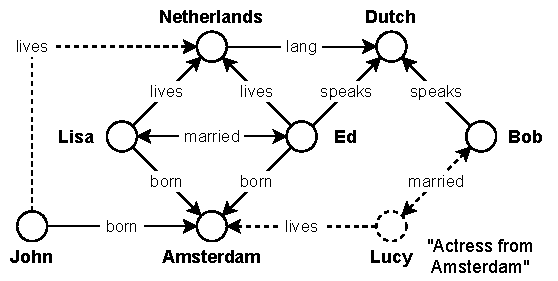
\includegraphics{1_introduction/example_kg}
    \caption{ Simple knowledge graph stating facts like "Ed speaks Dutch" or "Ed is married to Lisa". A pattern one might recognize in the graph structure could be that implication $born(X, amsterdam) => lives(X, netherlands)$ holds true most of the time. One might thus complement the graph by predicting the missing fact $lives(john, netherlands)$. The open world entity "Lucy" and the facts about her are not known during training time.}
    \label{fig:1_introduction/example_kg}
\end{figure}

Knowledge graphs are often manually crafted and may thus have missing facts about recent events or less important entities. Parts of this unrecorded knowledge can be derived from patterns in the graph structure. If, for example, 90\% of the people who live in Amsterdam also speak Dutch, one might assume that some person from Amsterdam, who is missing an associated language, speaks Dutch. Several approaches have achieved good results~\cite{Wang2017KnowledgeGE} for such \emph{knowledge graph completion} (KGC).

The problem becomes more complex when attempting to predict facts for entities that are not part of the graph. This scenario is known as \emph{open world scenario} with the unknown entities being called \emph{open world entities}. In contrast, the entities that are part of the graph and thus seen during training are called \emph{closed world entities}. A scenario that does not include handling of open world entities is referred to as \emph{closed world scenario}. Without further information about an open world entity, only vague assumptions can be made about it, e.g. a 10\% chance that it is a person, if 10\% of all closed world entities were persons. With additional information, however, like the entity's name or description, further assumptions can be made. The description "Actress from Amsterdam", for example, allows the conclusion that the entity is a person who lives in Amsterdam.

% based on short descriptions, Villmov et al. proposed OWE
% for CW they embed texts and graph into low dim vector spaces and learn mapping
% then can embed OW texts, map into graph space

Based on such textual entity annotations, Villmov et al. proposed an open-world extension for embedding-based knowledge graph completion models~\cite{Shah2019AnOE}. Embedding-based KGC models represent the graph in a low dimensional vector space that is trained such that embeddings of similar entities are close together while those of dissimilar ones are far apart~\cite{Wang2017KnowledgeGE}. As shown by Villmov et al. it is possible to train a mapping function that maps an open world entity's textual description into the graph embedding space and subsequently make predictions using the underling KGC model.

% requirement is graph embedding
% embedding based considered state of the art for KGC models for some time
% other approach towards KGC is symbolic
% recently, rule-based caught attention with good results (anyBURL)
% advantage of rule-based: human understandable

Prerequisite for the approach is an embedding-based KGC model, which does not seem to be a strong limitation since most state-of-the-art KGC models are embedding-based~\cite{Wang2017KnowledgeGE}. Besides embedding-based models, there also exist rule-based models that have received less attention in the past. Rule-based models find propositional rules that describe the structure of the graph, e.g. $ lives(X, amsterdam) => speaks(X, dutch) $. Their great advantage is that humans can understand the found rules that lead to a decision. Recently, Meilicke et al. argued that rule-based models were underestimated and have presented the rule-based model AnyBURL, which surpassed the embedding-based state-of-the-art models in many ways~\cite{Meilicke2019AnytimeBR}. They conclude that rule-based models should be considered in future research as well.

Following their suggestion, the goal of this thesis is to build an extension for rule-based knowledge graph completion models that uses textual annotations of entities to predict links in the knowledge graph, thus enabling open world prediction. Furthermore, it will be investigated whether these predictions are humanly comprehensible as one might hope on the basis of readable rules.


\section{Source Code}
\label{sec:1_introduction/1_source_code}
power source code available under MIT licence on GitHub
includes streamlit app
also, repos for experiments (power-experiment-*)

